% Chapter 3

\chapter{方案设计}

\section{概要}
设计要求是:用户输入一张图片后,可以得到相应的标注语句,了解图片语义;在用户输入一句话的时候,可以得到描述这一句话的图片,直观“感受”文字。

软件设计主界面使用python的tkinter包来制作。python是一个跨平台语言,用python制作方便产品在不同平台使用。界面中应当可以选择调动两个功能,分别是图片翻译为自然语言和语句翻译为图片。两个功能分别提前训练出成品模型,通过主界面按钮内嵌入的方法,调用对应模型进行计算。

\section{软件模型}
软件分为三个部分,第一部分是软件界面,需要实现简洁明了的操作功能,方便使用。

第二部分是图片标注功能。实现这一功能的模型通过image caption的模型进行训练,算法参照蒙特利尔大学Kevin Xu\upcite{xu2015show}提出的模型进行实现,并经过基于一个或多个数据集进行多个epoch的训练,比较选出表现较好的模型,嵌入到应用中使用。

第三部分是文本生成图片功能。实现这一功能的模型通过一个特殊的GAN模型进行训练,并且要加入后期图片处理算法,以骗过判别器并使其更加真实。这一模型参照卡耐基-梅隆大学Justin Johnson\upcite{Johnson_2018}提出的基于场景双GAN模型配合进行实现,并经过合适的数据集训练,得到表现较好的模型,嵌入到应用当中使用。

\section{变量符号与定义}
文中使用集合如下:
\begin{enumerate}[fullwidth,itemindent=2em,label=\arabic*.]
    \item $O$代表物品(object)的集合;
    \item $C$代表物品目录(catagory)的集合;
    \item $R$代表关系(relationship)的集合;
    \item $E$代表物品-关系-物品组成的边(edge)的集合。
\end{enumerate}

文中脚标定义如下:
\begin{enumerate}[fullwidth,itemindent=2em,label=\arabic*.]
    \item ${}_t$代表LSTM模型中的时序,${}_t$为当前时序,而${}_{t-1}$或${}_{t+1}$为前一或后一时序;
    \item $_f$代表任一函数(使用$f$指代)代入当前操作或模型;
    \item $v_i$在第二个算法中,代表GCN当前层级的节点编号,因为不讨论跨多层关系,所以脚标中不增加时序信息。
\end{enumerate}

文中小写字母对象定义如下:
\begin{enumerate}[fullwidth,itemindent=2em,label=\arabic*.]
    \item $s$指代集合$S$中的元素,其中$S$指代任一集合,如物品集合$O$等,他们通常和集合一起出现;
    \item $c$代表LSTM模型中的细胞(cell),记录细胞当前状态;
    \item $i$代表LSTM模型中的输入门(input),执行LSTM模型中的输入操作;
    \item $o$代表LSTM模型中的输出门(output),执行LSTM模型中的输入操作;
    \item $f$代表LSTM模型中的遗忘门(forget),选择LSTM细胞的部分状态丢失;
    \item $z$代表生成模型中为了骗过判别器、降低生成图片锐度增加的噪声。
\end{enumerate}

文中主要函数定义如下:
\begin{enumerate}[fullwidth,itemindent=2em,label=\arabic*.]
    \item $\phi$代表注意力机制;
    \item $\mathcal{L}$函数代表GAN模型中用作训练目标函数的损失函数;
    \item $f(S,z)$代表自然语言生成图像算法中的目标函数。
\end{enumerate}

\section{软件界面设计}
\subsection{软件例图}
对于预期的软件效果,我制作了原型图(图~\ref{fig:UIproto})进行示意。图中,应当出现英文的地方用英文示意,应当出现路径的地方用路径示意,而应当出现中文的地方和说明文字使用中文表述。
\begin{figure}[!htb]
    \centering
    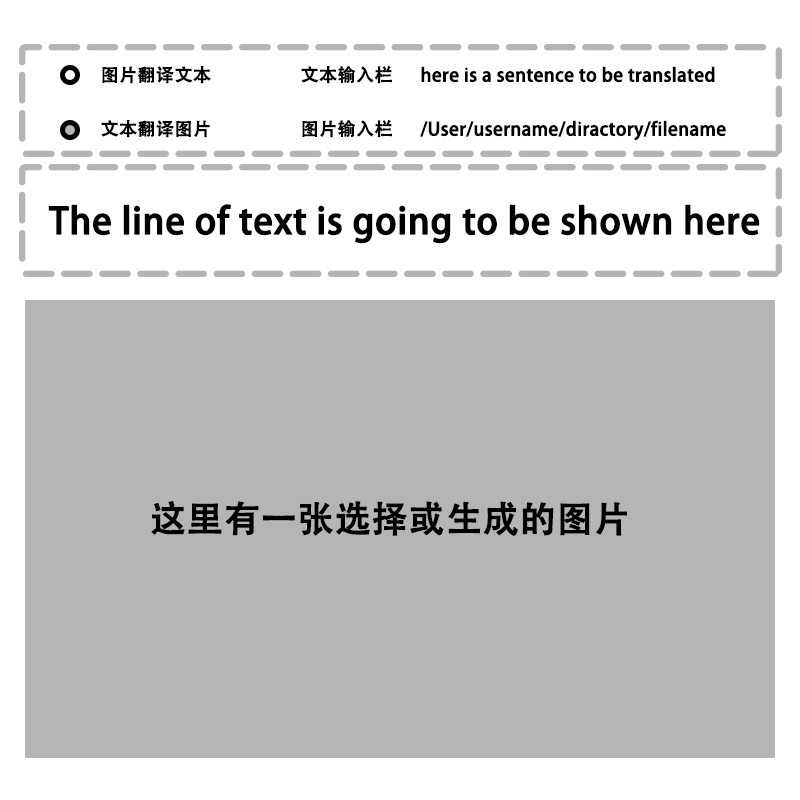
\includegraphics[width=0.8\textwidth]{figures/界面原型图.png}
    \caption{软件界面原型图}
    \label{fig:UIproto}
  \end{figure}

  其中,界面上方由一组两个单选选项的选择栏和两个数据输入栏组成。选项栏的作用是选择当前需要实现的功能,由“图片翻译语义”和“文本翻译图片”两个选项组成;数据输入栏分别是一个文本输入栏和一个文件选择栏,分别对应着文本和图片的输入选择。

  其下是一个明显的按钮,突出的设计可以让用户能轻易明白操作方法,也让用户更有仪式感,能感受到这一操作的划时代意义。

  最下方的大区域是输出区域,根据功能的不同可以输出不同的内容。在选择图像翻译语义功能时,会输出一句话,这一行文字和图片将一起显示,方便对比观察;在选择语义生成图像选项时,将输出生成的图片和原语句,也是为了方便用户观察与分享,表意清晰。

\subsection{软件开发模型}
对开发设计软件的过程,我选用了编码-修改模型\upcite{pressman2005software}。如图~\ref{fig:codenfix}所示,在这一模型中不进行计划与建模,先进行编码,调整至用户满意时,发布运行,在出现问题与更新时维护,直到软件生命周期结束为止。

本次软件设计开发的过程是要独立接触一个不熟悉的领域,对于开发者来说不易估计编码需要的时间。深度学习对初学者来说有一个难点:环境安装中很多细节难以把控;并且深度学习的学习过程需要使用多块显卡进行天级时长的训练过程,才可以得到结果。基于上述理由,我可以推测算法的实现需要比较长的时间,并且可能一次训练出的算法达不到理想的状态,需要调整模型、重复训练。

\begin{figure}[!htb]
    \centering
    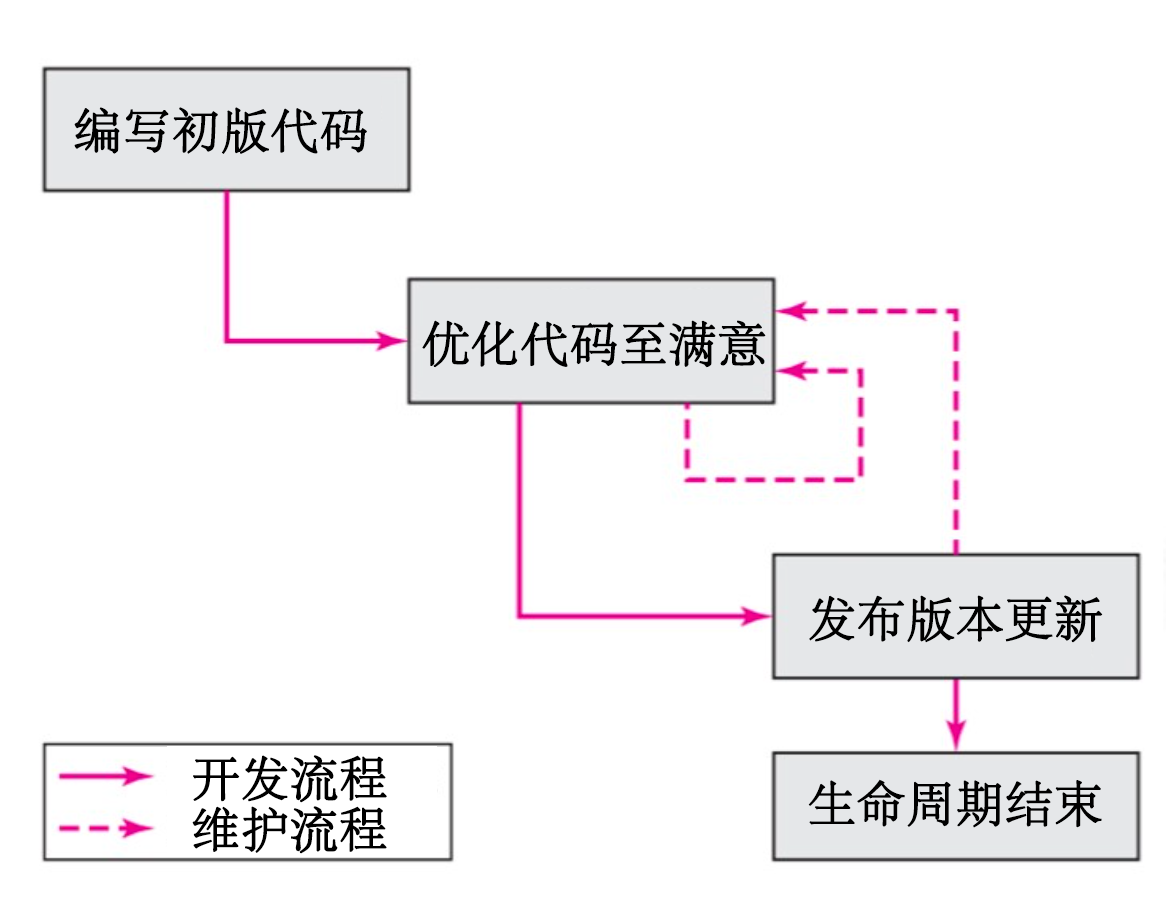
\includegraphics[width=0.6\textwidth]{figures/codeandfix.png}
    \caption{编码-修改模型的基本结构}
    \label{fig:codenfix}
\end{figure}

在设计的过程中,对我来说的难点的确是环境安装部分。需要的新虚拟容器因为电脑上旧有的项目擅自修改了环境变量,需要重新安装、整理环境,并且安装合适版本的环境,搭配当前系统,对开源项目进行修改、复现,并在此基础上进行改进。

另外,本软件的模型相对比较简单,是用户界面-调用模型的两层结构,难点在于模型的建立和调整。所以本设计非常适合使用编码-修改模型进行开发。

\section{软件功能设计}
功能部分分为图片标注功能以及文字生成图像功能,两个功能我使用了两个结构相对复杂的深度学习模型组合构架的算法,将在下面具体介绍。
 
\subsection{图片标注方法}
\subsubsection{算法整体模型}
在这一模型中,要使用LSTM模型进行训练,训练出的模型放在主函数的调用函数中,实现图片翻译为自然语言的功能。

这一模型主要流程由四步组成。

\begin{enumerate}[fullwidth,itemindent=2em,label=\arabic*.]
    \item 在模型中输入图片,作为输入信息;
    \item 由卷积神经网络提取图片信息,形成图片特征信息(即后文编码步骤);
    \item 由注意力机制(attention)对所提取的图片特征信息进行处理,加强或抑制部分区域,作为后续输入LSTM的输入信息——在不同时刻,注意力信号会受到上一次LSTM的输出信息的影响,即注意力信号作为LSTM神经元细胞的状态,受到输出词语的影响而改变(这也是后文的解码部分);
    \item LSTM最终输出文本,形成最后的结果。
\end{enumerate}

\subsubsection{编码部分}
第一步,要对训练集中的标注编码,形成特征向量。词典中已经预先确定了$K$个词语,对于每一行标注$y_i$,可以将其通过词典序号,将句子映射成输入向量,每一个元素的位置意义是序号,即图片相关的类别,数字则是关联度。编码之后生成向量$\textbf{y}_i$,一起构成输入矩阵。
$$y = {\textbf{y}_1, \textbf{y}_2, ..., \textbf{y}_C}, \textbf{y}_i\in \mathbb{R}^K$$

第二步,对图片编码。使用一个卷积神经网络(Convolutional Neural Network, CNN)对图片的特征进行提取,从而形成图片编码。编码好的图片,后续会作为注释向量$\textbf{a}$使用。
$$a = \{\textbf{a}_1, \textbf{a}_2, ... , \textbf{a}_L\}, \textbf{a}_i \in \mathcal{R}^D$$

\subsubsection{解码部分}
解码部分使用的技术是LSTM,即长短期记忆模型。解码后生成的是标注文本,在预测最后一个词的时候,需要背景向量、前一时刻的隐藏层向量、前一时刻的词。这一部分实用的LSTM模型结构,由图示意出。
\begin{figure}[!htbp]
    \centering
    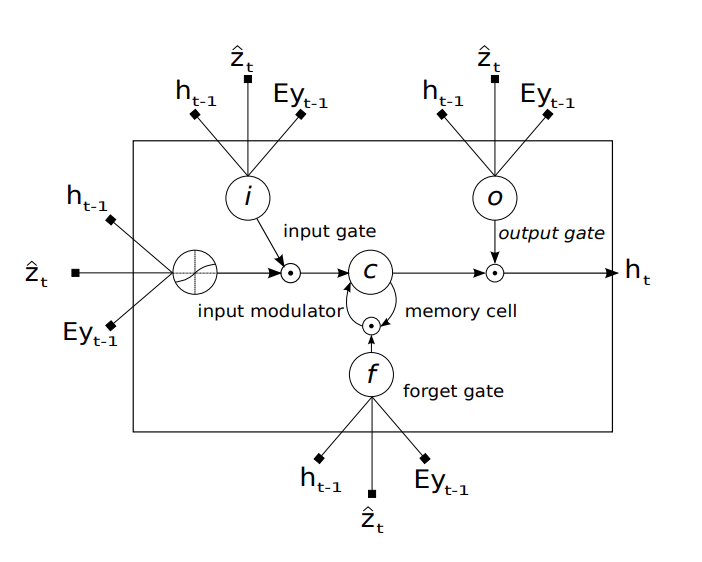
\includegraphics[width=0.8\textwidth]{figures/lstm_token.png}
    \caption{解码LSTM神经元细胞模型结构图}
    \label{fig:lstm_tokenize}
\end{figure}

背景向量$\hat{z}_t$由注意力机制函数和图片注释向量计算得出,并且与时序$t$有关,随时序推进而变化。相当于是有选择地传输图片注释向量中的信息,是图片信息的动态表达。

确定一个注意力机制函数$\phi$来计算$t$时刻的背景向量$\hat{z}_t$。对于输入的图片注释信息,为了推测这一位置是否是正确的注意力集中点,在式\eqref{eq:归一a}中定义一个可以归一化的参数$\alpha_{t,i}$来表示在$t$时刻,位置$i$是正确关注点的置信度。
\begin{equation}
    e_{t,i}=f_{att}(\textbf{a}_i,\textbf{h}_t)
\end{equation}
\begin{equation}
    \label{eq:归一a}
    \alpha_{t,i}=\frac{\exp e_{t,i}}{\sum_{k=1}^{L}\exp e_{t,k}}
\end{equation}

计算置信度时需要用到$f_{att}$函数,这一函数定义为一个“硬”机会注意力机制函数。
这一机会注意力机制的“软”版本由Bahdanau\upcite{bahdanau2014neural}提出,仿照这个机制可以提出硬版本函数。

现在定义$s_t$为模型为了生成第$t$个单词所选择的注意力区域。其中,$s_t$的第$i$项是开关函数,此项置1时,当前模型生成打你是第i个单词。
现设定多次伯努利分布的参数${\alpha_i}$,将背景向量视为随机事件,则有:
\begin{equation}
    p(s_{t,i} = 1|s_{j<t}, \textbf{a}) = \alpha_{t,i}
\end{equation}

计算出权重之后,即可使用注意力机制函数计算出背景向量$\hat{z}_t$:
\begin{equation}
    \label{eq:bgvector}
    \hat{z}_t=\phi(\textbf{a}_i,\alpha_i)
\end{equation}
\begin{equation}
    \hat{z}_t = \sum_i s_{t,i}\textbf{a}_i
\end{equation}
一个“软”估计得算法即如式\eqref{eq:softatt}的方法计算出。但是,还可以提出一种“硬”估计的
\begin{equation}
    \begin{aligned}
        &&\phi(\{\textbf{a}_i\},\{\alpha_i\})&= \mathbb{E}_{p(s_t\mid a)} [\hat{z}_t] \\
        && & =\sum_{i=1}^L \alpha_{t,i} \cdot \textbf{a}_i \\
    \end{aligned}
    \label{eq:softatt}
\end{equation}

现在定义一个概率的对数函数,计为$L_s$,作为模型的优化目标;对于训练的目标参数$W$,$L_s$函数就是优化目标。则可以推导得其下界为式\eqref{eq:hard1}所示,从而得到最终训练梯度为式\eqref{eq:lstmtar}
\begin{equation}
    \begin{aligned}
        && L_s &= \sum_s p(s, \textbf{a}) \log p(\textbf{y}\mid {s }, \textbf{a} ) \\
        && & \le \log \sum_sp(s, \textbf{a}) p(\textbf{y}\mid {s }, \textbf{a} ) \\
        && & = \log p(\textbf{y}, \textbf{a})
    \end{aligned}
    \label{eq:hard1}
\end{equation}
\begin{equation}
    \frac{\partial L_s}{\partial W} = \sum_s p(s \mid a) [\frac{\partial \log p(\textbf{y}\mid {s }, \textbf{a} )}{\partial W} + \log p(\textbf{y}\mid {s }, \textbf{a} ) \frac{\partial \log p(\textbf{y}, \textbf{a})}{\partial W} ]
    \label{eq:lstmtar}
\end{equation}

其中有
\begin{equation}
    \tilde{s}_t \sim Multinoulli_L({\alpha_i})
    \label{eq:stdistribute}
\end{equation}

则
\begin{equation}
    \frac{\partial L_s}{\partial W} \approx \frac{1}{N} \sum_{i=1}^{n} [\frac{\partial \log p(\textbf{y}\mid \tilde{s}^n, \textbf{a} )}{\partial W} + \log p(\tilde{s}^n \mid \textbf{a} ) \frac{\partial \log p(\textbf{y}, \textbf{a})}{\partial W} ]
    \label{eq:lstmtar2}
\end{equation}

这里的函数$\phi$是利用了“软”确定注意力机制(Deterministic “Soft” Attention),这一机制算法可以稍为简易地作出注意力正确位置的判断,可以作出计算,用于判断下一个词的注意力位置;并且,这个函数的目的是计算注意力,而非前文从提取注意力。可以将$\hat{z}_t$的期望值$\mathbb{E} [\hat{z}_t]$作为其取值,带入计算,即设定$\phi$函数为式\eqref{eq:softatt}中的计算方法。

从式\eqref{eq:lstmtar}中,可以看出优化函数$L_s$由基于蒙特卡罗方法多次采样逼近梯度的方式,对式\eqref{eq:stdistribute}遵从多次伯努力分布的注意力区域位置进行采样,测算优化函数。在这个时序数据中,为了消除,使用滑动平均基线的方法\upcite{10.5555/2074022.2074088},令基线的对数更新比例如式\eqref{eq:baseline}所示。
\begin{equation}
    \label{eq:baseline}
    b_k = 0.9 \times b_{k-1} + 0.1 \times \log p(\textbf{y} \mid \tilde{s}_k, a)
\end{equation}

最终得到的“硬”注意力函数如式\eqref{eq:hard3}所示。
\begin{equation}
    \frac{\partial L_s}{\partial W} \approx \frac{1}{N} \sum_{i=1}^N\left[\frac{\partial \log p(\textbf{y}\mid \tilde{s}^n,\textbf{a})}{\partial W} + \lambda_r[]\log p(\textbf{y}\mid \tilde{s}^n,\textbf{a})-b] \frac{\partial \log p(\tilde{s}^n \mid \textbf{a})}{\partial W} +\lambda_e\frac{\partial H[\tilde{s}^n]}{\partial W}\right]
    \label{eq:hard3}
\end{equation}

将其代回式\eqref{eq:bgvector}中的$\phi$函数,即可得出${\textbf{a}_i}$由“硬”选择注意力集中位置的参数${\alpha_i}$加权后的取样结果。

解决了背景向量的问题,可以开始训练LSTM模型了。对于这个模型,需要进行初始化,确定其中图~\ref{fig:lstm_tokenize}标注的传入隐状态$h_0$及其内部初始环境$c_0$。取标注向量的平均,作为初始的状态,进行操作。即:
$$\textbf{c}_0 = f_{init,c}\left(\frac{1}{L}\sum_{i=1}{L}\textbf{a}_i\right)$$
$$\textbf{h}_0 = f_{init,c}\left(\frac{1}{L}\sum_{i=1}{L}\textbf{a}_i\right)$$
%\subsubsection{代码实现模块}

\subsection{自然语言生成图片方法}
这一模型主要是用通过场景生成图像的GAN模型来训练,得到的模型放在主函数的调用函数中,实现自然语言生成图片的功能。

\subsubsection{图片生成模型}
生成图片的总体的算法流程如算法~\ref{algo:sg2im-all}所示,分为三个大步骤:GCN确定场景布局,确定图像边框布局,级联优化网络(Cascade Refinement Network)\upcite{chen2017photographic}。

\begin{algorithm}[H]
    \setstretch{1.5} % 代码间行距设定
    \SetAlgoLined
    \vspace{2em}
    \algorithmicrequire 自然语言短句$S$,噪声$z$\\
    \algorithmicensure 生成图片$\hat{I} = f(G,z)$\\
    %\Function{a}{b}
    $O,E \gets $提取(物品)元素和(位置)关系$($生成语义树$(S))$\;
    $G \gets $构成物品关系图$(O,E)$\;
    $\textbf{Layout} \gets $GCN$(G)$\;
    $I \gets Generate(Layout)$ \;
    $\hat{I} \gets CRN(I)$\;
    %\EndFunction
    \caption{图片生成方法}
    \label{algo:sg2im-all}
\end{algorithm}

\vspace{2em}
第一步的图卷积网络(GCN)需要输入场景关系图,它是由自然语言经过简单处理后得到的。场景关系图满足下列条件:
$$O={o_1,...,o_n},o_i \in C$$
$$E \subseteq O \times R \times O =\{(o_i,r_{ij},o_j)\mid i,j \in \mathbb{N}^\star\}, r \in R$$

图卷积网络可以沿着场景图的关系(边)$e_i$,计算出图中各个物体$o_i$的嵌入向量$ \textbf{v}_i$。其单层局部结构如图~\ref{fig:gcn}所示,这张图示意了图卷积网络的每一层之间,向量如何更新迭代。

\begin{figure}[!htb]
    \centering
    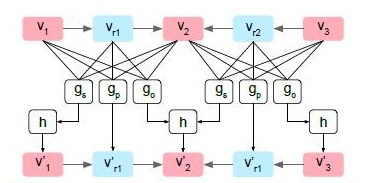
\includegraphics[width=0.9\textwidth]{figures/gcn.png}
    \caption{图卷积神经网络(GCN)单层结构图}
    \label{fig:gcn}
\end{figure}
图~\ref{fig:gcn}中$v_i$代表物体向量,而$v_{ri}$代表关系向量。其中涉及了三个物品$o_1, o_2, o_3$和两组关系$(o_1,r_1,o_2), (o_2,r_2,o_3)$。这些向量需要经过三个函数,分别是$g_o, g_p, g_s$,其中$g_o, g_s$的值需要作为候选变量,参与到调和函数$h$中,最终决定更新后的物体向量。

关系向量的更新比较简单,它遵从式\eqref{eq:vrupdate}。
\begin{equation}
    v'_r = g_p(v_i,v_r,v_j)
    \label{eq:vrupdate}
\end{equation}

而图中的物体元素则更为复杂一些。要考虑每一个元素作为它参与的所有关系中的角色,而计算出它的更新向量。对于每一个物体向量$o_i$,它对应下列两个候选向量,供调和函数调用。其中$V_i^o $代表了所有$o_i$作为关系中被指向的点所在关系所生成的候选向量集合,反之 $V_i^s$ $o_i$代表了所有$o_i$作为关系中指向起点所在关系所生成的候选向量集合。
$$V_i^s = \{g_s(o_i, r, o_j)\mid (o_i, r, o_j)\in E\}$$
$$V_i^o = \{g_o(o_j, r, o_i)\mid (o_j, r, o_i)\in E\}$$

随后,我们可以通过式\eqref{eq:viupdate}中的调和函数更新物体向量$ v_i $。
\begin{equation}
    v'_i = h(V_i^s, V_i^o)
    \label{eq:viupdate}
\end{equation}

生成的图像还需要两个额外的生成模型进行优化,以得到平滑效果更好的生成图像。图像的平滑程度是评价生成图像质量的重要标准之一。

第一部分中,我们得到了最终得到了每个物体的高级特征表达向量(关系的特征表达向量主要作为隐藏值影响物体的特征向量计算)。在第二部分中,则需要测算每一个物体的框架位置。

对于上一环节得到的每一个物体的特征表达向量$\hat{v}_i$,我们分别将它传入蒙板回归网络(Mask Regression Network)和框回归网络(Box Regression Network),分别求出其在画布上的形状和位置。最终得到形状蒙板$\hat{m}$和$\hat{b}$:
$$\hat{m} \sim M \times M$$
$$\hat{b} = (x_0,y_0,x_1,y_1)$$

将$\hat{m} $和物体特征向量 $v_i $按照元素序逐一将值相乘,得到物体的形状与样式,再将其缩放,使其可以代入$\hat{b}$所规定的框架中,则可以得到这一物体的形状、位置与大小。

第三部分则是将在画布上的物体拼合,组成一幅新的“图像”。这个图像要求所有的元素都在其中对此,

\subsubsection{鉴别模型}
我们生成了两个鉴别网络模型,用作与前述生成模型进行对抗。

第一个判别器$D_{img}$是对整个$f$ 函数结果,即生成图片$\hat{I}$进行判别。这个判别器的损失函数是:
\begin{equation}
    \mathcal{L}_{D_{img}} = \mathbb{E}_{x\sim p_{real}} [\log D(x)] + \mathbb{E}_{x\sim p_{fake}} [1-D(x)]
    \label{eq:lossdimg}
\end{equation}
其中,$x\sim p_{real}$指训练集中提供的真实图片$I$,而$x\sim p_{fake}$则是指生成图片$\hat{I}=f(g)$。生成模型函数$f$的训练目标是最小化判别器得出的$\mathcal{L}_{D_{img}}$值。

$f, \mathcal{L}_{D_{img}}$函数组成的GAN网络模型,保证了图片整体的真实性和平滑性,与\cite{isola2017image}中的判别器性质类似。

当然,在生成模型第二部分生成的物体图片要单独进行训练,这就需要一个使用另一个判别器${D_{obj}}$来进行对每个物体的图像判别。但是物体的图像大小可能会与原图不相同,但这是不影响图片生成效果的,所以在判别之前需要用双线性插值\upcite{bilinear}的方法将图片变换处理为相同的大小,以减小大小对判别带来的过拟合。 

除此之外,判别器还要做一项特殊的工作。与以往的GAN网络不同,它是一道保险装置,希望再不输入物体类别,仅输入生成图像时,将物体判别为正确的分类。在这一方面,判别器和生成器都希望正确类别的置信度尽量高,以保证其在\cite{odena2017conditional}中提到的判别标准(Auxiliary Classifier)中的可识别性。

经过以上恰当的双GAN模型训练与保险机制,可以得到可用的图片生成器$f$。

\section{本章小结}
本章具体地介绍了这一设计中所包含的设计细节及其理论依据,并确定了软件构架的结构,为完成代码构建和实验设计打下了基础。

本章中,确定了以python语言的tkinter库来写界面,保证界面简单简介易懂;用CNN和LSTM技术,基于注意力的方法,通过编码-解码的流程来完成图片标注功能;用基于位置场景的方法,由GNN和两个判别器构成的GAN模型来分步生成图片,最后生成合成图片的方法来实现由文本生成图片的功能。

在下一章里,我会继续记述实验的过程及其表现。
%{\songti \bfseries 宋体加粗} {\textbf{English}}

%{\songti \itshape 宋体斜体} {\textit{English}}

%%%{\songti \bfseries \itshape 宋体粗斜体} {\textbf{\textit{English}}}

%\section{编译}
%本模板必须使用XeLaTeX + BibTeX编译,否则会直接报错。 本模板支持多个平台,结合sublime/vscode/overleaf都可以使用。